\documentclass[11pt]{article}
%Gummi|061|=)
\title{\textbf{project active-memory}}
\author{santex@cpan.org}
\date{}
\usepackage{graphicx}
\begin{document}

\maketitle

\section{Before you start}

Try to mentally step back for a second and imagine you standing infront of a 100 gigabyte data chunk format JSON,\\
rock solid painted in black.\\\\
Your existence depends on finding the little data Nugget who lives in GigaByte 52.17
you never seen the thing bevor,
what do you do.



\section{AI-micro-structures}
They are called like that because they have multiple properties some are related to the nugget you still searching. The name giving properties come from the genetic way the data is organised.


\begin{figure}[htp]
\centering
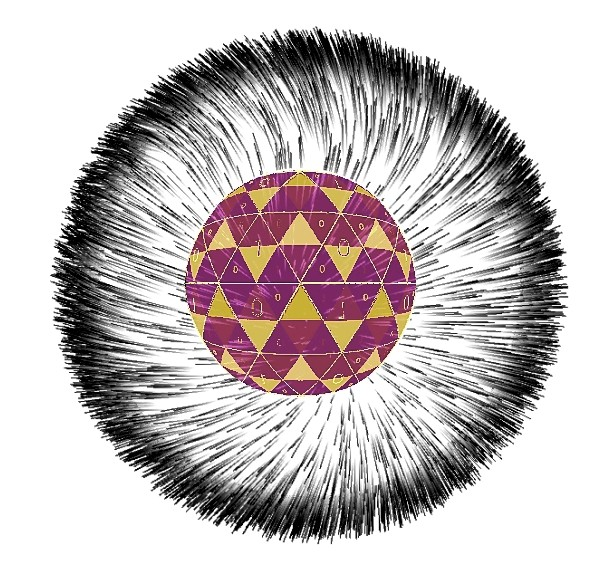
\includegraphics[scale=0.29]{./image/artee-0.jpg}
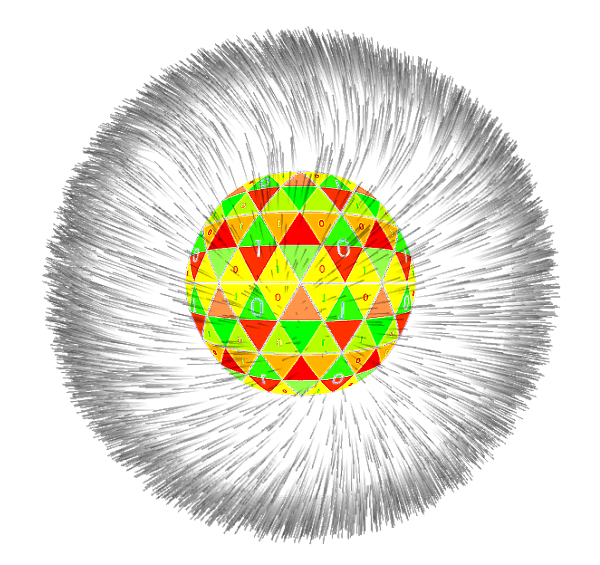
\includegraphics[scale=0.29]{./image/artee-1.png}
\caption{}
\label{}
\end{figure}


\section{Optimized data-surface}
\begin{figure}[htp]
\centering
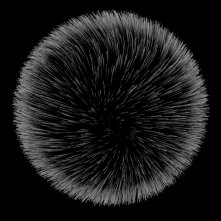
\includegraphics[scale=0.9]{./image/query-surface.jpg}
\end{figure}
\subsection{Data Restructure}

\begin{itemize}
\item Each knot in the data structure is identified
\item same query distance for each knot in the structure
\item generations for revisions
\item scanning for knowledge
\item uncontrolled data-evolution by matrix exchange and 
fitness comparrison
\end{itemize}
\subsection{Fitness}


\begin{itemize}
\item querying based on a matrix within a semantic domain
\item data fitness based on query matrix


\end{itemize}

\subsection{Data States}

\begin{itemize}

\label{item any mix of states}
\item growing
\item unknown
\item semantically signed



\section{Concept Theory}

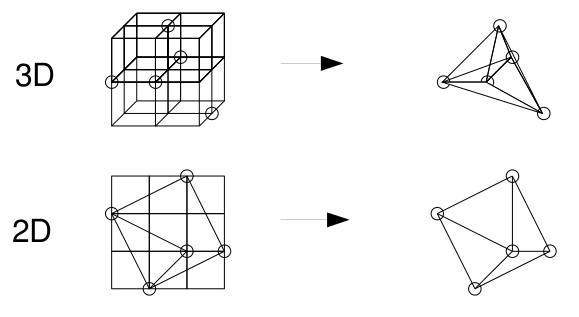
\includegraphics[scale=0.65]{image/research-base-002.png}



\section{Concept applied on Data}
\begin{figure}[htp]
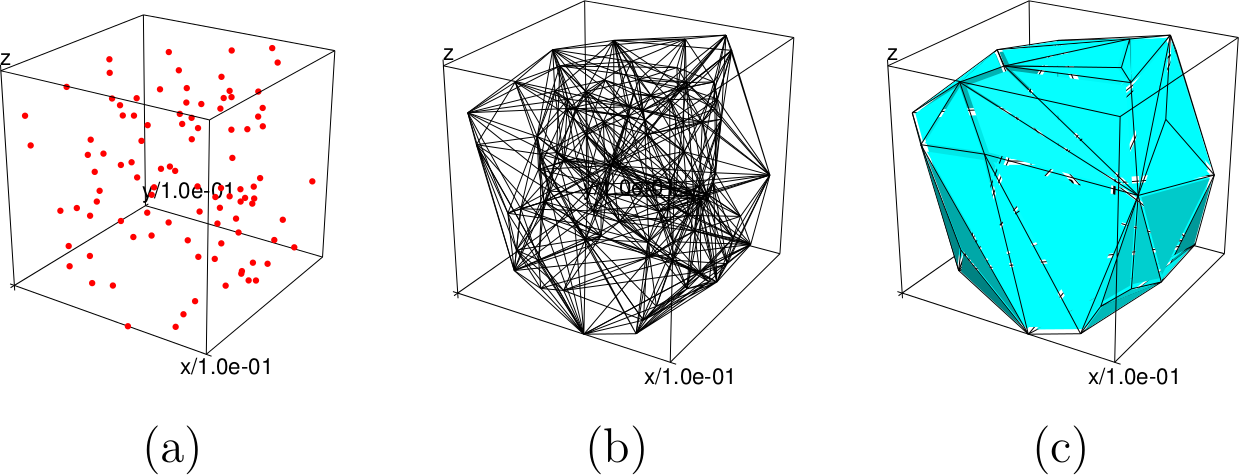
\includegraphics[scale=0.32]{image/research-base-001.png}
\end{figure}



\section{Coding it}

It will work by adding a closed unit (mesh + matrix + reactor) in front of a CouchDb
The unit uses a array of algorithms to bring light to the data map it and restructure to harmonised entity most likely we will have in the
common toolbox (linux,perl, couchdb, POE, RamDisk, JSON)
core toolbox (tetgen, meshlab, CPAN::[Math,AI,Algorithm,Statistics]).
The matrix we start with will be able to express
(static,liquid,common,unique,dominant) semantic signing for data.


\section{Concept applied on Query}
\begin{figure}[htp]
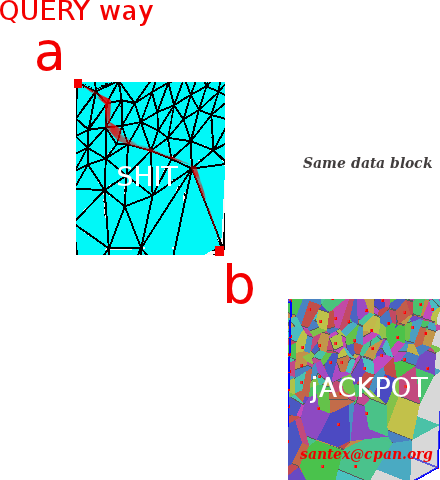
\includegraphics[scale=0.43]{image/research-base-003.png}

\subsection{Unknown Data with tet-gen}
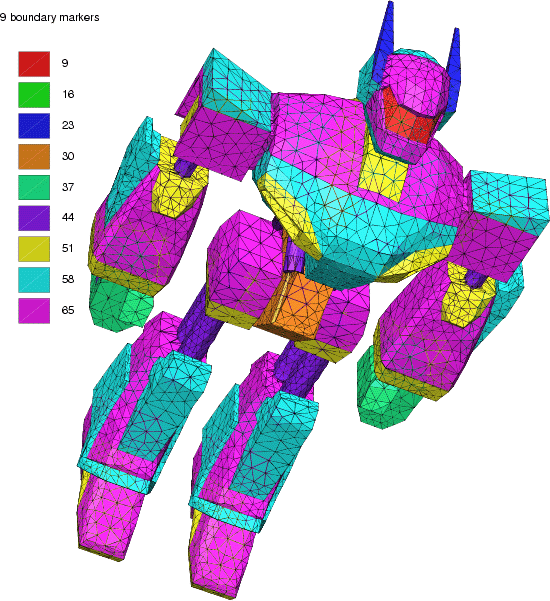
\includegraphics[scale=0.3]{image/unknow-robot.png}
\end{figure}

\begin{itemize}
\begin{figure}[htp]
\section{Entities and Emergence}


\item Micro-structure
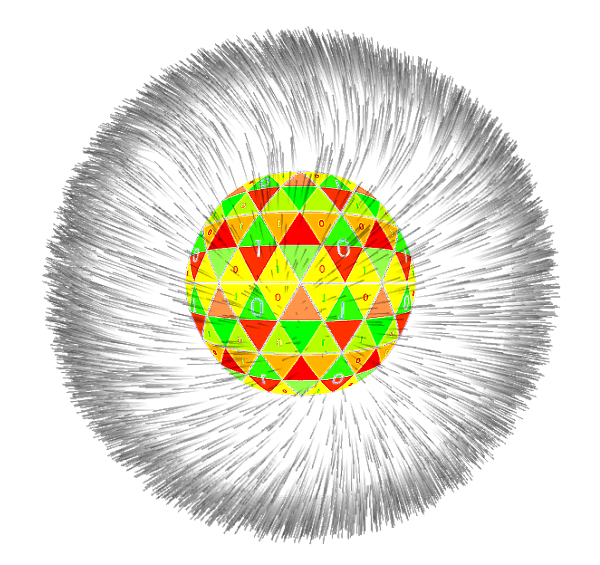
\includegraphics[scale=-0.3]{image/artee-1.png}
\\
\\
\\
\\
\\
\\
\\
\\
\\
\\
\item Procreation
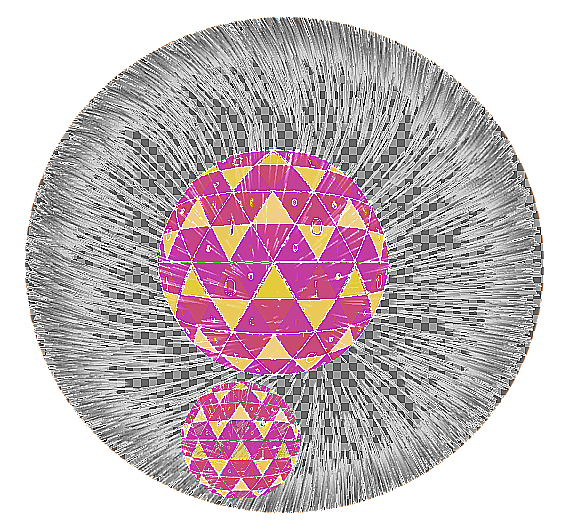
\includegraphics[scale=0.5]{image/artee-procreation.png}
\item Symbiotic
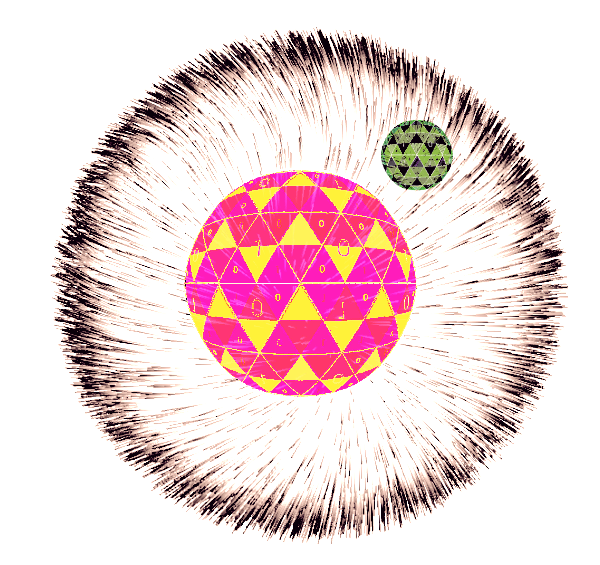
\includegraphics[scale=-0.2]{image/artee-symbiosis.png}
\end{figure}

\end{itemize}
\end{itemize}

\end{document}

